\chapter{Introduction}\label{chap:introduction}

Today's mobile Internet is no longer controlled only by a signular stakeholder, e.g. a standard body or a telecommunications company.
Rather, the interests of a multitude of stakeholders, e.g. application developers, hardware vendors, cloud operators, and network operators, collide during the development and operation of applications in the mobile internet. 
Each of these stakeholders considers different \glspl{KPI} to be important and attempts to optimise scenarios in its favour. 

One example of such a scenario are \emph{Signalling Storms}~\cite{Huawei2011} in the mobile Internet, with one of the largest occurring in Japan in 2012\footnote{\url{https://www.techinasia.com/docomo-outage}, Accessed: November, \(21^{st}\) 2015} due to the release and fast uptake of a free instant messaging application.
The application traffic generated by the application caused a high number of connections between to the Internet being created and torn-down.
This resulted in a high number of signalling messages in the mobile network, causing overload and a loss of service for 2.5 million users over 4 hours.
While the network operator suffers the largest impact of this signalling overload it does not control the application.
Thus the network operator can not change the application traffic characteristics to generate less network signalling traffic. 
The stakeholders who could prevent or at least reduce such behaviour, i.e. application developers or hardware vendors, have no direct benefit from modifying their products in such a way.
This is an example where a clash of stakeholder interests negatively impacts the network performance for all participants.

The goal of this monograph is to provide an overview over the complex structures of stakeholder relationships in today's Internet applications.
To this end, we study different scenarios where such stakeholder interests clash and suggest methods where stakeholder tradeoffs can be optimised for all participants.
If such such an optimisation is not possible or attempts at it might lead to adverse effects, we discuss the causes.

In the remainder of this chapter we first discuss the stakeholders considered in this work in \refsec{sec:introduction:considered_stakeholders}.
Then, in \refsec{sec:introduction:scientific_contribution} we provide an overview over the scientific contributions of this thesis.
Finally, \refsec{sec:introduction:outline} provides an outline of this monograph.

\section{Scope}\label{sec:introduction:considered_stakeholders}

In this section we introduce the stakeholders considered in the remainder of this monograph.
\reffig{fig:introduction:stakeholders} shows the major stakeholders and their interactions.

\begin{figure}
\centering
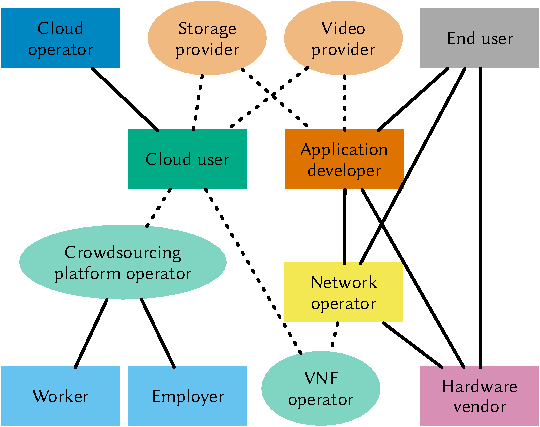
\includegraphics{figures/stakeholders}
\caption{Stakeholder interactions considered in this monograph. Solid lines show stakeholder interactions, dotted lines show \emph{is-a} relationships.}\label{fig:introduction:stakeholders}
\end{figure}

First, we consider the \emph{network operator}.
The network operator owns, manages and operates a mobile network.
By manipulating network configuration, the operator can influence the connection state of \gls{UE}, resulting in changes of power drain, i.e. battery life, of the \gls{UE} produced by the hardware vendor and reduced signalling load in the components of its mobile network.

The \emph{application provider} develops and deploys applications and is interested in increasing the \gls{QoE} for the user, in order to attract a large user base.
Additional considered \glspl{KPI} are cost, for example incurred due to use of compute or network resources in \gls{IaaS} or \gls{PaaS} scenarios.
Design and configuration of applications have impact on traffic patterns which result in signalling traffic in the network of the mobile network operator and also influence the power drain of the \gls{UE} of the hardware vendor.

%TODO: Video Provider, Storage Provider

\glspl{UE} are developed and sold by \emph{hardware vendors}.
While they theoretically implement standards proposed by the \gls{3GPP} in order to establish connectivity with mobile networks, in reality vendors are free to deviate from standard, in order increase own \glspl{KPI}.
One example of such a deviation from a standard are proprietary fast dormancy mechanisms~\cite{GSM2010} implemented by some hardware vendors.
These algorithms reduce power drain be disconnecting the \gls{UE} earlier from the network, in order to reduce power drain and increase end user \gls{QoE}.
However, this has the consequence of increased signalling in the network of the network operator and can result in increased page load times, i.e. decreased \gls{QoE} from the end users point of view.

\emph{End users} employ \glspl{UE} to execute applications in the network of network operator. 
They are usually interested in increasing their \gls{QoE}, i.e. by increasing the battery life of their \gls{UE} or increasing satisfaction during video playback over the network.

\emph{Cloud operators} provides services, i.e. compute, storage, or network resources, to cloud users according to specified \glspl{SLA} for monetary compensation. 
They attempt to reduce the costs to operate infrastructure, e.g. by reducing power drain, in order to increase revenue while still satisfying the \gls{SLA} negotiated with the cloud users.
Resources provided by cloud operators are purchased by \emph{cloud users}.
They attempt to provide the best possible service to their own customers while reducing the number of required resources provided by the cloud operator, in order to reduce cost of operation. In this monograph we consider two exemplary cloud users, which will be discribed in the following:

A \emph{\gls{NFV} operator} uses virtualised resources obtained from a cloud operator to provide virtualised network services to other stakeholders.
In the example considered in this thesis, the \gls{NFV} operator uses cloud compute resources in order to provide a \gls{GGSN} to a mobile network operator.
The \glspl{KPI} of the \gls{NFV} operator are satisfying the \gls{SLA} with the mobile network operator and reducing the use of compute resources of the cloud operator.

The second considered cloud user is the \emph{crowdsourcing platform operator} who uses cloud resources in order to provide a crowd sourcing platform.
The crowdsourcing platform operator in turn has to consider the requirements of its two main stakeholders:
The \emph{crowdsourcing employer} requires a set of microtasks to be completed in a small amount of time, in order to use the generated results in future business processes. 
\emph{Crowdsourcing workers} complete microtasks for a set amount of money.
They are interested in completing as many tasks as possible and reduce their idle time, in order to increase their income.

The interactions of this stakeholders result in complex interactions, which are studied in this thesis.
The next section introduces the considered interactions and provides an overview over the scientific contributions provided by this monograph.

\section{Scientific Contribution}\label{sec:introduction:scientific_contribution}
This monograph studies the interactions between different stakeholders in three, partially overlapping, scenarios in order to paint a broad picture of today's interlocking network and application ecosystem.

\begin{figure}
\centering
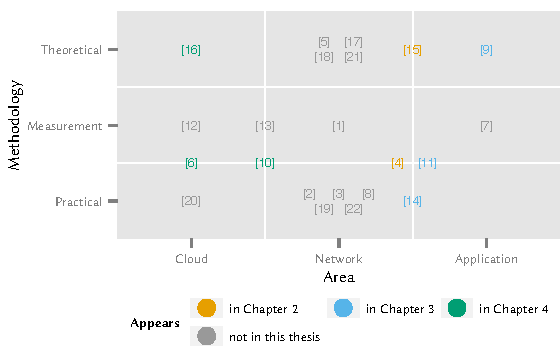
\includegraphics{figures/publications}
\caption{Contribution of this work as a classification of the research studies conducted by the author}\label{fig:introduction:publications}
\end{figure}

In \reffig{fig:introduction:publications} we classify the areas of research as well as scientific method used in relation to the chapter of this monograph.
The x-axes shows the impacted areas of research, i.e. topics related to the mobile network, the application domain or cloud technologies.
The y-axes details the applied scientific method.
The theoretical area includes methods queueing theory, mean value analysis and analysis of random variables.
Measurements were performed using testbeds and simulation studies were performed using \gls{DES}.

Annotations of are used to highlight scientific publication who's content contributes to the respective chapters.

The first contribution of this monograph is a study of the impact of mobile application traffic on mobile communication networks, especially considering the current network configuration.
TWe study the impact of different traffic types, both from real-world applications and synthetic traffic distributions, and study the potential of network parameter optimisation as a mean to reduce signalling traffic.

As a second contribution, we provide models for two popular applications, i.e. Video Streaming and Cloud File Synchronisation, thus enabling the study of the impact of different mechanisms implemented in said applications.
%For the Video Streaming application we use a simulation in order to compare \glspl{KPI} for all stakeholders in this scenario.
We show that the Streaming mechanism allows the most flexible configuration and can provide a Pareto optimal results for all pairs of metrics.
However, further study shows that in fact no pareto optimal value exists which satisfies the \glspl{KPI} of all participating stakeholders.
Furthermore, we provide parameterisable \gls{QoE} models for different user groups.
Finally, for the Cloud File Synchronisation we compare different upload scheduling algorithms and find that both the Size based algorithm as well as the Time based algorithm can be used to specify a tradeoff between the different considered \glspl{KPI}.

As a third contribution, we discuss the impact of resource dimensioning and management schemes in cloud environments.
To this end, we first study the performance of a power conservation mechanism for cloud environments using a queueing model.
We derive guidelines for selecting Pareto optimal results regarding both waiting time before a job can begin processing and power drain of the cloud.
Then, we discuss a mechanism to reduce cost for cloud users by disabling compute instances while still allowing configurable \glspl{SLA} and evaluate this mechanism using a queueing simulation.
Finally, we present a mechanism to dimension worker numbers in a human cloud scenario which can be used to ensure satisfaction the key stakeholders of a crowdsourcing platform operator.

\section{Outline of Thesis}\label{sec:introduction:outline}

In \refchap{chap:network} we study the impact of mobile network configuration settings on participating stakeholders, i.e. mobile network operators, hardware vendors, and users.
We present an algorithm to infer power drain and signalling messages caused by a given application traffic measurement.
Then, we perform application traffic measurements and discuss general traffic characteristics before applying the introduced algorithm to the measurements.
We generalise our results by introducing a theoretical model for power drain and signalling messages for arbitrary \gls{IID} traffic distributions.

\refchap{chap:application} focusses on the impact of applications design and algorithm choice by the application developers on the other stakeholders.
We study two prominent applications in today's Internet: Video Streaming and Cloud File Sychronisation.
%video transmission mechanisms hatte einen neuen namen?
For Video Streaming, we study the impact of different video transmission mechanisms and parameter configurations on energy consumption of the \gls{UE}, signalling in the mobile network and resource consumption at the application developer using a \gls{DES}.
%auch das hatte einen anderen namen
Furthermore, we study provide a queueing model for video streaming algorithms and derive a parameterised \gls{QoE} model.
Next, we discuss different scheduling algorithms for Cloud File Synchronisation services.
Using data obtained from large scale, testbed based~\cite{Chun2003} measurements, we implement a simulation model in order to investigate \glspl{KPI} for the relevant stakeholders.  

In \refchap{chap:cloud} we study resource allocation strategies in the cloud and evaluate in which management decisions of the cloud platform operators impact the other stakeholders.
First, we consider a energy saving scheme where a cloud operator scales the number of available servers according to the available load.
We introduce a queueing model and perform a performance evaluation in order to study optimal parameter settings.
Then, we consider the role of a cloud user renting virtual machines in the cloud in order to provide a service to users on the example of a virtualised network operator.
We analyse traffic characteristics and use them as input for a simulation model of a virtualised \gls{GGSN}.
Then, we evaluate the impact of different virtual server setups and scaling configurations.
Finally, we consider resource allocation in human clouds.
Based on data obtained from a commercial crowdsourcing provider, we extract characteristic distributions and apply it as input two both an analytic queueing model as well as a simulation model and derive dimensioning guidelines for the crowdsourcing provider.

Finally, \refchap{chap:conclusion} provides a summary of the major contributions of this work and provides an outlook on future potential research directions.